\documentclass[12pt,letterpaper]{article}
\usepackage[utf8]{inputenc}
\usepackage[spanish]{babel}
\usepackage{graphicx}
\usepackage[left=2cm,right=2cm,top=2cm,bottom=2cm]{geometry}
\usepackage{graphicx} % figuras
% \usepackage{subfigure} % subfiguras
\usepackage{float} % para usar [H]
\usepackage{amsmath}
%\usepackage{txfonts}
\usepackage{stackrel} 
\usepackage{multirow}
\usepackage{enumerate} % enumerados
\renewcommand{\labelitemi}{$-$}
\renewcommand{\labelitemii}{$\cdot$}
% \author{}
% \title{Caratula}
\begin{document}

% Fancy Header and Footer
% \usepackage{fancyhdr}
% \pagestyle{fancy}
% \cfoot{}
% \rfoot{\thepage}
%

% \usepackage[hidelinks]{hyperref} % CREA HYPERVINCULOS EN INDICE

% \author{}
\title{Caratula}

\begin{titlepage}
\begin{center}
\large{UNIVERSIDAD PRIVADA DE TACNA}\\
\vspace*{-0.025in}
\begin{figure}[htb]
\begin{center}

\includegraphics[width=8cm]{./Imagenes/logo}
\end{center}
\end{figure}
\vspace*{0.15in}
INGENIERIA DE SISTEMAS \\

\vspace*{0.5in}
\begin{large}
TITULO:\\
\end{large}

\vspace*{0.1in}
\begin{Large}
\textbf{INFORME DE LABORATORIO N01 - Elaboración de Dashboards en Power BII} \\
\end{Large}

\vspace*{0.3in}
\begin{Large}
\textbf{CURSO:} \\
\end{Large}

\vspace*{0.1in}
\begin{large}
INTELIGENCIA DE NEGOCIOS\\
\end{large}

\vspace*{0.3in}
\begin{Large}
\textbf{DOCENTE(ING):} \\
\end{Large}

\vspace*{0.1in}
\begin{large}
 Patrick Cuadros Quiroga\\
\end{large}

\vspace*{0.2in}
\vspace*{0.1in}
\begin{large}

\begin{flushleft}
Alumno: \\
Rodriguez Mamani, Juan Rigoberto 		\hfill	(2017057862) \\
\end{flushleft}
\end{large}
\end{center}

\end{titlepage}


\tableofcontents % INDICE
\thispagestyle{empty} % INDICE SIN NUMERO
\newpage
\setcounter{page}{1} % REINICIAR CONTADOR DE PAGINAS DESPUES DEL INDICE

\section{Actividad 01: Conectar a SQL Server desde Power BI Desktop } 

Iniciamos Power BI Desktop y conectamos con la Base de Datos AdventureWorks2017 de SQLServer

	\begin{center}
	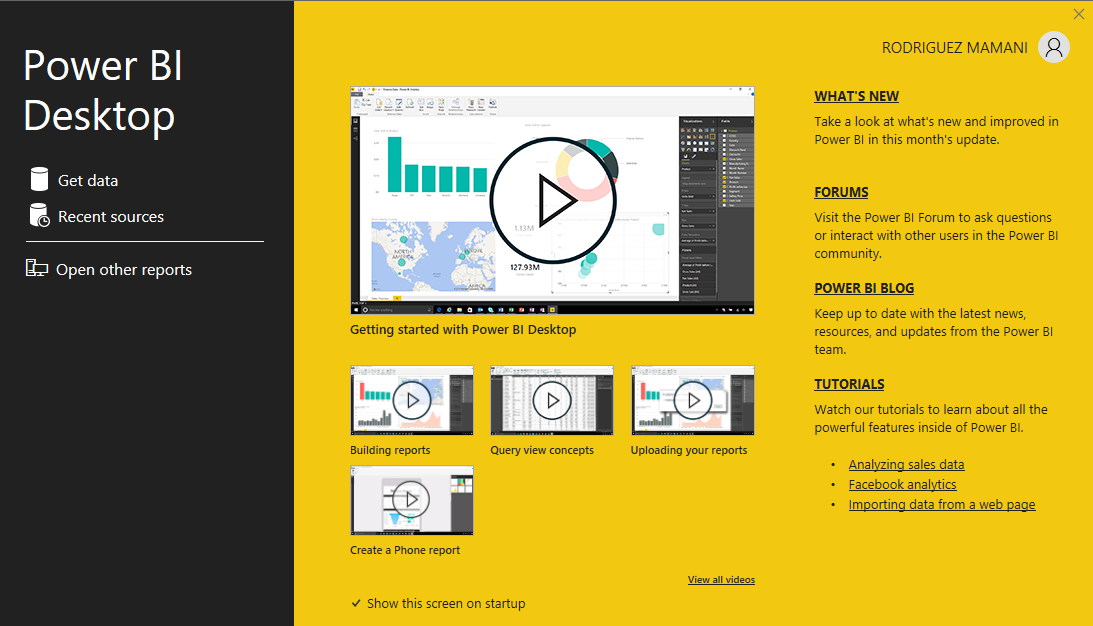
\includegraphics[width=17cm]{./Imagenes/imagen1}
	\end{center}	

	\begin{center}
	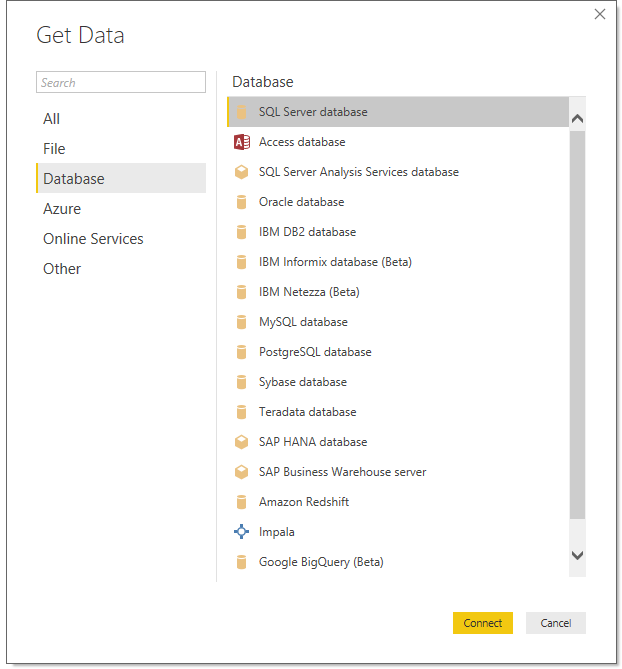
\includegraphics[width=17cm]{./Imagenes/imagen2}
	\end{center}

	\begin{center}
	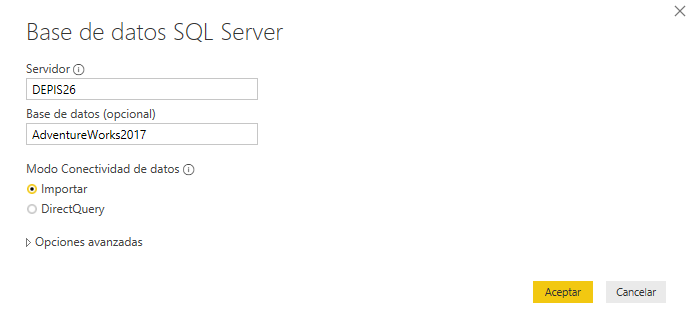
\includegraphics[width=17cm]{./Imagenes/imagen3}
	\end{center}

	\begin{center}
	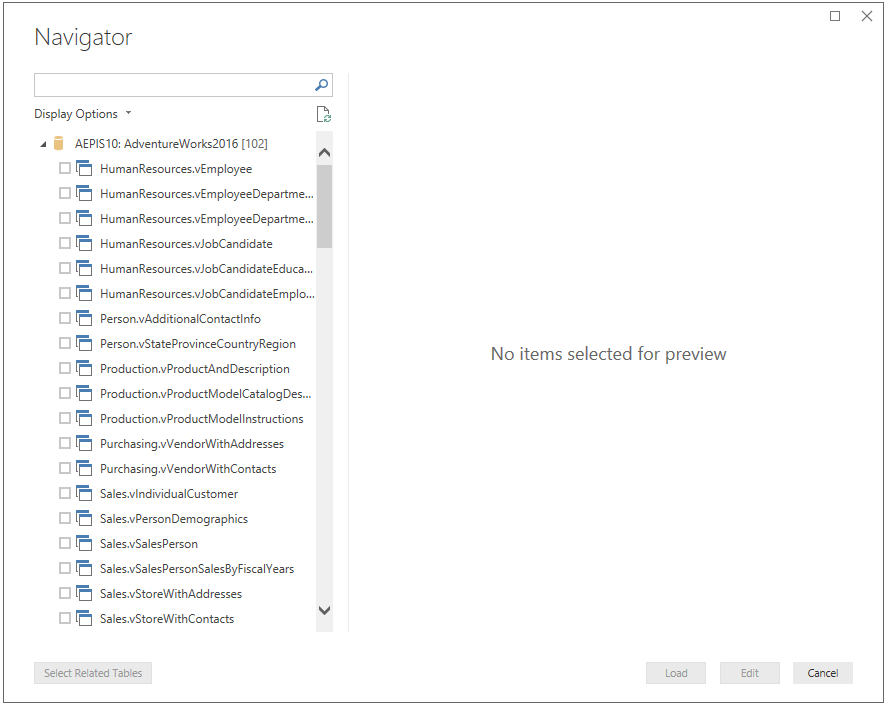
\includegraphics[width=17cm]{./Imagenes/imagen4}
	\end{center}
\section{Actividad 02: Adicionar Gráficos al Reporte} 

Creamos los diferentes graficos solicitados con los datos de la Base de Datos AdventureWorks2017
	\begin{center}
	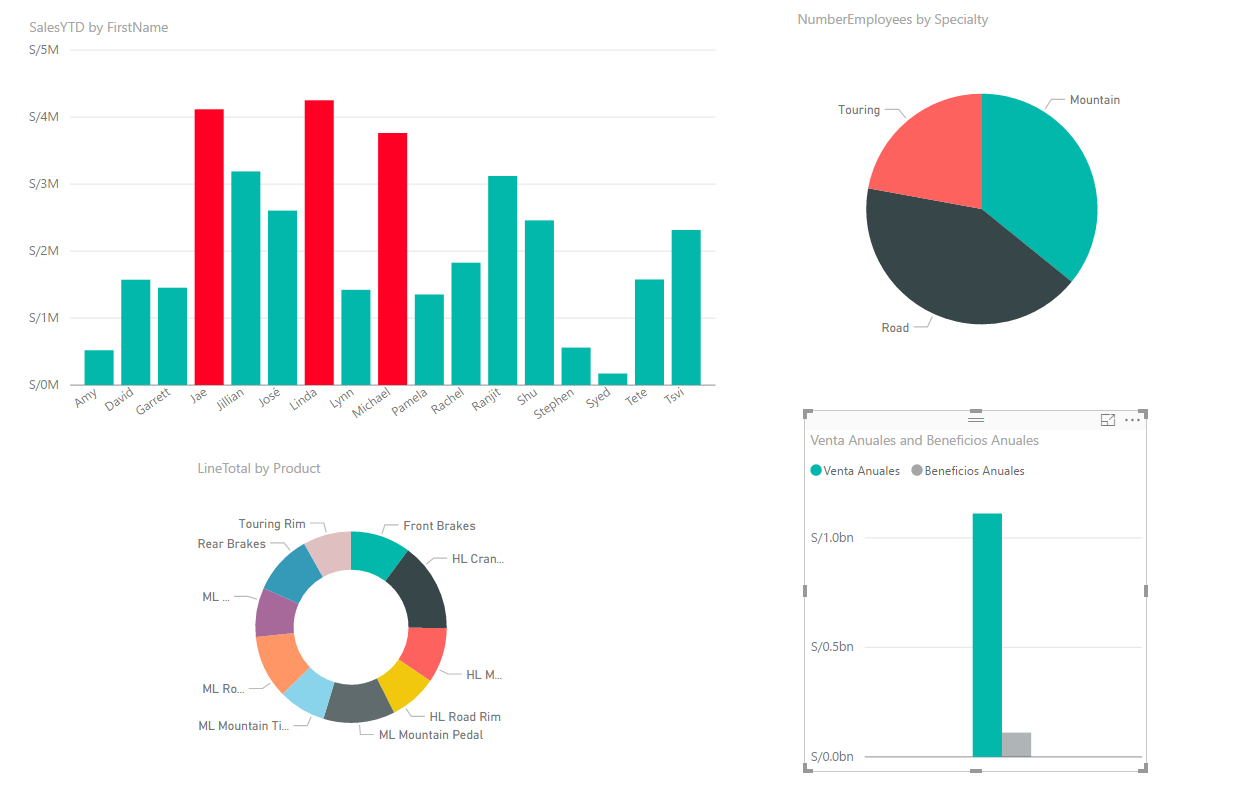
\includegraphics[width=17cm]{./Imagenes/imagen5}
	\end{center}	
\section{Actividad 03: Publicar el reporte en el portal de Power BI} 

Finalizado la creacion de graficos, procedemos a publicar nuestro trabajo en el portal de PowerBI

	\begin{center}
	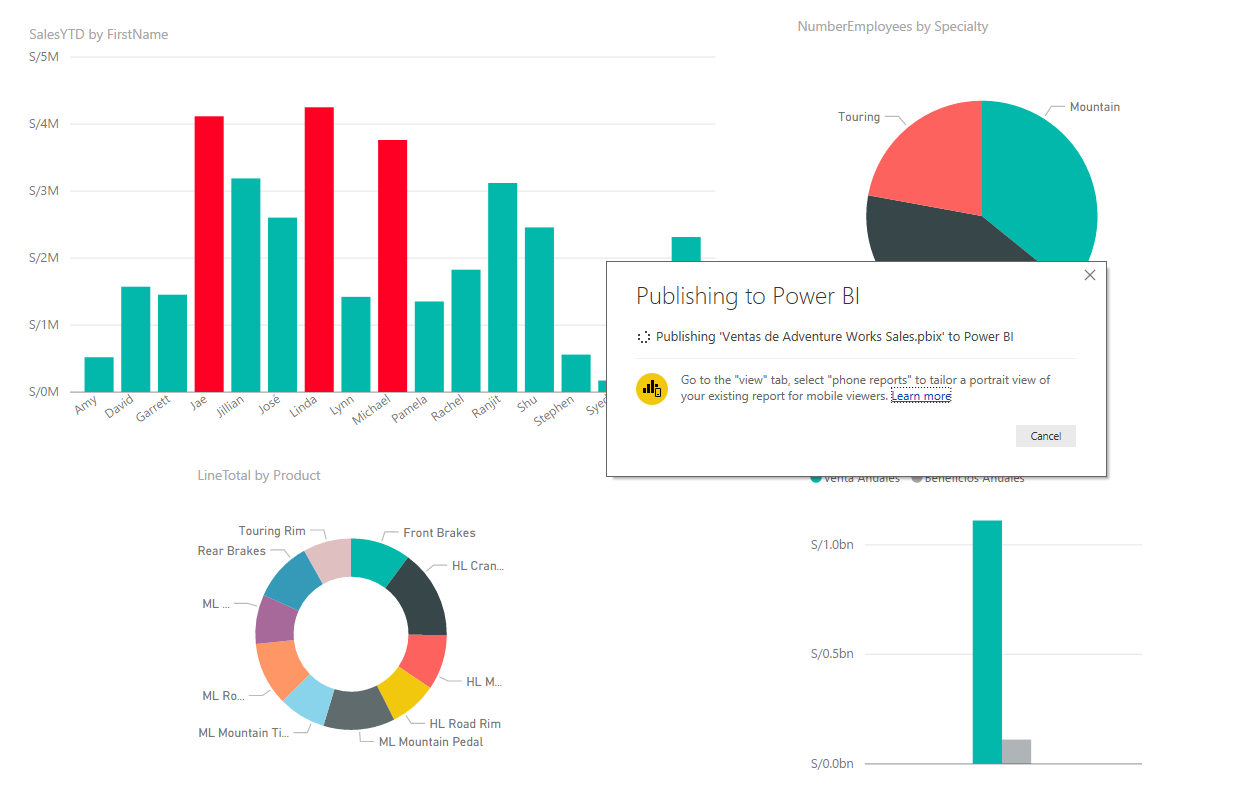
\includegraphics[width=17cm]{./Imagenes/imagen6}
	\end{center}	

	\begin{center}
	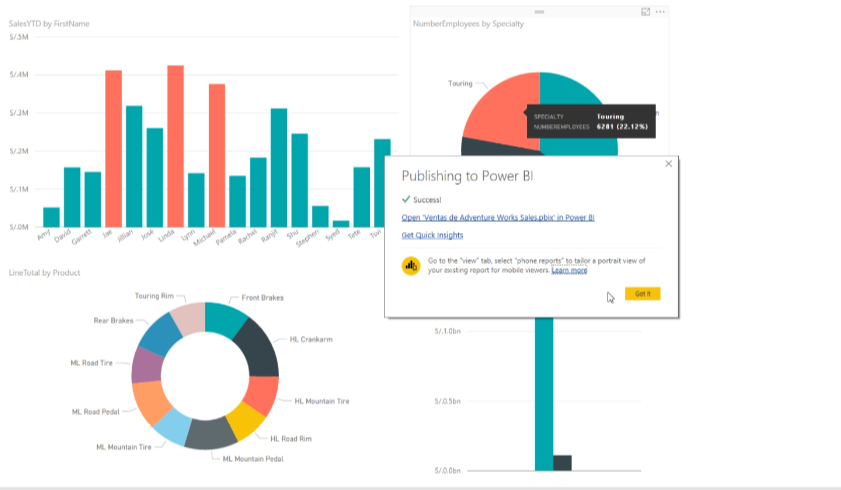
\includegraphics[width=17cm]{./Imagenes/imagen7}
	\end{center}	

\end{document}
